% GNUPLOT: LaTeX picture with Postscript
\begingroup
  \makeatletter
  \providecommand\color[2][]{%
    \GenericError{(gnuplot) \space\space\space\@spaces}{%
      Package color not loaded in conjunction with
      terminal option `colourtext'%
    }{See the gnuplot documentation for explanation.%
    }{Either use 'blacktext' in gnuplot or load the package
      color.sty in LaTeX.}%
    \renewcommand\color[2][]{}%
  }%
  \providecommand\includegraphics[2][]{%
    \GenericError{(gnuplot) \space\space\space\@spaces}{%
      Package graphicx or graphics not loaded%
    }{See the gnuplot documentation for explanation.%
    }{The gnuplot epslatex terminal needs graphicx.sty or graphics.sty.}%
    \renewcommand\includegraphics[2][]{}%
  }%
  \providecommand\rotatebox[2]{#2}%
  \@ifundefined{ifGPcolor}{%
    \newif\ifGPcolor
    \GPcolortrue
  }{}%
  \@ifundefined{ifGPblacktext}{%
    \newif\ifGPblacktext
    \GPblacktexttrue
  }{}%
  % define a \g@addto@macro without @ in the name:
  \let\gplgaddtomacro\g@addto@macro
  % define empty templates for all commands taking text:
  \gdef\gplbacktext{}%
  \gdef\gplfronttext{}%
  \makeatother
  \ifGPblacktext
    % no textcolor at all
    \def\colorrgb#1{}%
    \def\colorgray#1{}%
  \else
    % gray or color?
    \ifGPcolor
      \def\colorrgb#1{\color[rgb]{#1}}%
      \def\colorgray#1{\color[gray]{#1}}%
      \expandafter\def\csname LTw\endcsname{\color{white}}%
      \expandafter\def\csname LTb\endcsname{\color{black}}%
      \expandafter\def\csname LTa\endcsname{\color{black}}%
      \expandafter\def\csname LT0\endcsname{\color[rgb]{1,0,0}}%
      \expandafter\def\csname LT1\endcsname{\color[rgb]{0,1,0}}%
      \expandafter\def\csname LT2\endcsname{\color[rgb]{0,0,1}}%
      \expandafter\def\csname LT3\endcsname{\color[rgb]{1,0,1}}%
      \expandafter\def\csname LT4\endcsname{\color[rgb]{0,1,1}}%
      \expandafter\def\csname LT5\endcsname{\color[rgb]{1,1,0}}%
      \expandafter\def\csname LT6\endcsname{\color[rgb]{0,0,0}}%
      \expandafter\def\csname LT7\endcsname{\color[rgb]{1,0.3,0}}%
      \expandafter\def\csname LT8\endcsname{\color[rgb]{0.5,0.5,0.5}}%
    \else
      % gray
      \def\colorrgb#1{\color{black}}%
      \def\colorgray#1{\color[gray]{#1}}%
      \expandafter\def\csname LTw\endcsname{\color{white}}%
      \expandafter\def\csname LTb\endcsname{\color{black}}%
      \expandafter\def\csname LTa\endcsname{\color{black}}%
      \expandafter\def\csname LT0\endcsname{\color{black}}%
      \expandafter\def\csname LT1\endcsname{\color{black}}%
      \expandafter\def\csname LT2\endcsname{\color{black}}%
      \expandafter\def\csname LT3\endcsname{\color{black}}%
      \expandafter\def\csname LT4\endcsname{\color{black}}%
      \expandafter\def\csname LT5\endcsname{\color{black}}%
      \expandafter\def\csname LT6\endcsname{\color{black}}%
      \expandafter\def\csname LT7\endcsname{\color{black}}%
      \expandafter\def\csname LT8\endcsname{\color{black}}%
    \fi
  \fi
    \setlength{\unitlength}{0.0500bp}%
    \ifx\gptboxheight\undefined%
      \newlength{\gptboxheight}%
      \newlength{\gptboxwidth}%
      \newsavebox{\gptboxtext}%
    \fi%
    \setlength{\fboxrule}{0.5pt}%
    \setlength{\fboxsep}{1pt}%
\begin{picture}(6480.00,6480.00)%
    \gplgaddtomacro\gplbacktext{%
      \csname LTb\endcsname%%
      \put(645,748){\makebox(0,0)[r]{\strut{}2.5}}%
      \csname LTb\endcsname%%
      \put(645,1238){\makebox(0,0)[r]{\strut{}3.0}}%
      \csname LTb\endcsname%%
      \put(645,1727){\makebox(0,0)[r]{\strut{}3.5}}%
      \csname LTb\endcsname%%
      \put(645,2217){\makebox(0,0)[r]{\strut{}4.0}}%
      \csname LTb\endcsname%%
      \put(645,2707){\makebox(0,0)[r]{\strut{}4.5}}%
      \csname LTb\endcsname%%
      \put(645,3197){\makebox(0,0)[r]{\strut{}5.0}}%
      \csname LTb\endcsname%%
      \put(645,3686){\makebox(0,0)[r]{\strut{}5.5}}%
      \csname LTb\endcsname%%
      \put(645,4176){\makebox(0,0)[r]{\strut{}6.0}}%
      \csname LTb\endcsname%%
      \put(645,4666){\makebox(0,0)[r]{\strut{}6.5}}%
      \csname LTb\endcsname%%
      \put(645,5156){\makebox(0,0)[r]{\strut{}7.0}}%
      \csname LTb\endcsname%%
      \put(645,5645){\makebox(0,0)[r]{\strut{}7.5}}%
      \csname LTb\endcsname%%
      \put(645,6135){\makebox(0,0)[r]{\strut{}8.0}}%
      \csname LTb\endcsname%%
      \put(845,464){\makebox(0,0){\strut{}2.5}}%
      \csname LTb\endcsname%%
      \put(1335,464){\makebox(0,0){\strut{}3.0}}%
      \csname LTb\endcsname%%
      \put(1824,464){\makebox(0,0){\strut{}3.5}}%
      \csname LTb\endcsname%%
      \put(2314,464){\makebox(0,0){\strut{}4.0}}%
      \csname LTb\endcsname%%
      \put(2804,464){\makebox(0,0){\strut{}4.5}}%
      \csname LTb\endcsname%%
      \put(3294,464){\makebox(0,0){\strut{}5.0}}%
      \csname LTb\endcsname%%
      \put(3783,464){\makebox(0,0){\strut{}5.5}}%
      \csname LTb\endcsname%%
      \put(4273,464){\makebox(0,0){\strut{}6.0}}%
      \csname LTb\endcsname%%
      \put(4763,464){\makebox(0,0){\strut{}6.5}}%
      \csname LTb\endcsname%%
      \put(5253,464){\makebox(0,0){\strut{}7.0}}%
      \csname LTb\endcsname%%
      \put(5742,464){\makebox(0,0){\strut{}7.5}}%
      \csname LTb\endcsname%%
      \put(6232,464){\makebox(0,0){\strut{}8.0}}%
      \csname LTb\endcsname%%
      \put(2804,2609){\rotatebox{-43}{\makebox(0,0){\strut{}$\sin^2 \theta_{23} = 0.4$}}}%
      \csname LTb\endcsname%%
      \put(3783,3588){\rotatebox{-43}{\makebox(0,0){\strut{}$\sin^2 \theta_{23} = 0.5$}}}%
      \csname LTb\endcsname%%
      \put(4763,4568){\rotatebox{-43}{\makebox(0,0){\strut{}$\sin^2 \theta_{23} = 0.6$}}}%
    }%
    \gplgaddtomacro\gplfronttext{%
      \csname LTb\endcsname%%
      \put(153,3490){\rotatebox{-270}{\makebox(0,0){\strut{}$P(\cj{\nu}_\mu \to \cj{\nu}_e)$ (\%)}}}%
      \csname LTb\endcsname%%
      \put(3587,185){\makebox(0,0){\strut{}$P(\nu_\mu \to \nu_e)$ (\%)}}%
      \csname LTb\endcsname%%
      \put(5844,6164){\makebox(0,0)[r]{\strut{}Normal hierarchy}}%
      \csname LTb\endcsname%%
      \put(5844,5978){\makebox(0,0)[r]{\strut{}Inverted hierarchy}}%
      \csname LTb\endcsname%%
      \put(5844,5792){\makebox(0,0)[r]{\strut{}Vacuum}}%
      \csname LTb\endcsname%%
      \put(5844,5606){\makebox(0,0)[r]{\strut{}$\delta_\text{CP} = -\pi$}}%
      \csname LTb\endcsname%%
      \put(5844,5420){\makebox(0,0)[r]{\strut{}$\delta_\text{CP} = -\pi/2$}}%
      \csname LTb\endcsname%%
      \put(5844,5234){\makebox(0,0)[r]{\strut{}$\delta_\text{CP} = 0$}}%
      \csname LTb\endcsname%%
      \put(5844,5048){\makebox(0,0)[r]{\strut{}$\delta_\text{CP} = \pi/2$}}%
    }%
    \gplbacktext
    \put(0,0){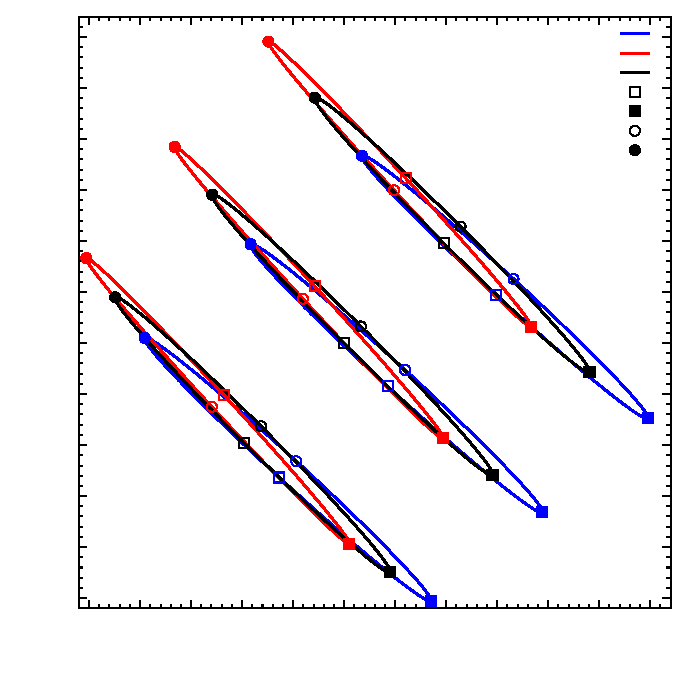
\includegraphics{pics/base_ball}}%
    \gplfronttext
  \end{picture}%
\endgroup
